%
% introduction.tex
%
% Copyright (C) 2022 by Universidade Federal de Santa Catarina.
%
% GNSS Networks Based on Small Satellites
%
% This work is licensed under the Creative Commons Attribution-ShareAlike 4.0
% International License. To view a copy of this license,
% visit http://creativecommons.org/licenses/by-sa/4.0/.
%

%
% \brief Introduction chapter.
%
% \author Gabriel Mariano Marcelino <gabriel.mm8@gmail.com>
%
% \version 0.0.0
%
% \date 2019/11/30
%

\chapter{Introduction} \label{ch:introduction}

Este trabalho tem como proposta o estudo, verificação de viabilidade e implementação de uma rede de um Sistema Global de Navegação por Satélite (\textit{Global Navigation Satellite System}, GNSS\nomenclature{\textbf{GNSS}}{Global Navigation Satellite System.}) baseada em satélites de pequeno porte, considerando especialmente os nanossatélites, ou em específico os CubeSats.

Os satélites de pequeno porte vêm crescendo de forma exponencial nos últimos anos, como pode ser visto na \autoref{fig:cubesat-launches} onde têm-se o número de lançamentos anuais de nanossatélites desde 1998, e o número previsto até 2025.

\begin{figure}[!ht]
    \begin{center}
        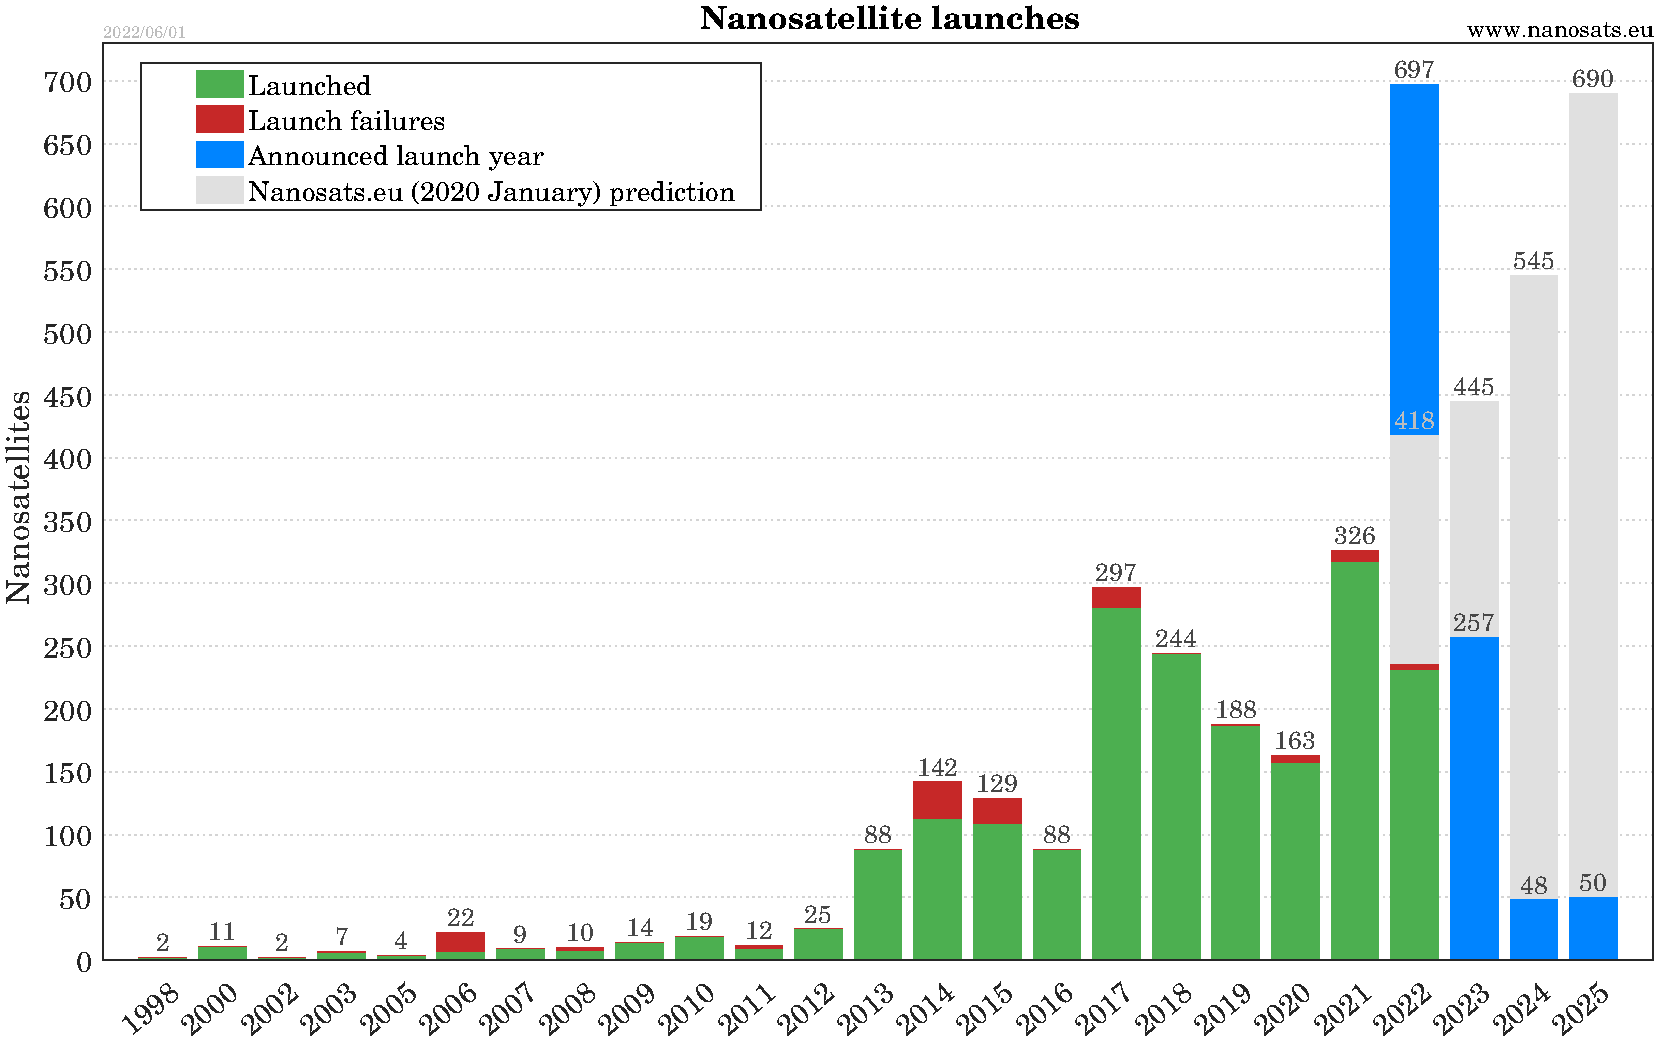
\includegraphics[width=\columnwidth]{figures/Nanosats_years_2022-06-01}
        \caption{Nanosatellite launches (2022/06/01) \cite{nanosatseu}.}
        \label{fig:cubesat-launches}
    \end{center}
\end{figure}

Com um custo consideravelmente menor, devido principalmente a utilização de órbitas mais baixas do tipo LEO\nomenclature{\textbf{LEO}}{Low Earth Orbit} (Low Earth Orbit) e de componentes COTS\nomenclature{\textbf{COTS}}{Commercial Off-The-Shelf}, vem se tornando cada vez mais fácil desenvolver e colocar este tipo de satélite em operação no espaço.

Um padrão que dominou o mercado de nanossatélites é o padrão CubeSat \cite{cds}, que normatiza várias características físicas para esses tipos de satélites. Este padrão, além de padronizar os subsistemas espaciais disponíveis no mercado, também normatiza os lançadores, o que faz com que se reduza o custo de lançamento de um nanossatélite, sendo um dos maios custos dentro deste tipo de projeto.

\section{Constellations}

Juntamente com a ascenção dos CubeSats, a constelações de pequenos satélites vêm surgindo e crescendo nos últimos anos. O baixo custo desse tipo de satélite junto com um grande recente crescimento do número de lançamentos também vêm facilitando a criação e implantação de constelações de pequenos satélite em baixa órbita. Com dezenas ou até centenas de satélites em órbita, é possível obter uma cobertura praticamente constante e sobre todo o território mundial. O gráfico da \autoref{fig:constellations} apresenta a situação das principais constelações de nanossatélites que já estão em operação e que estão em planejamento para implantação.

\begin{figure}[!ht]
    \begin{center}
        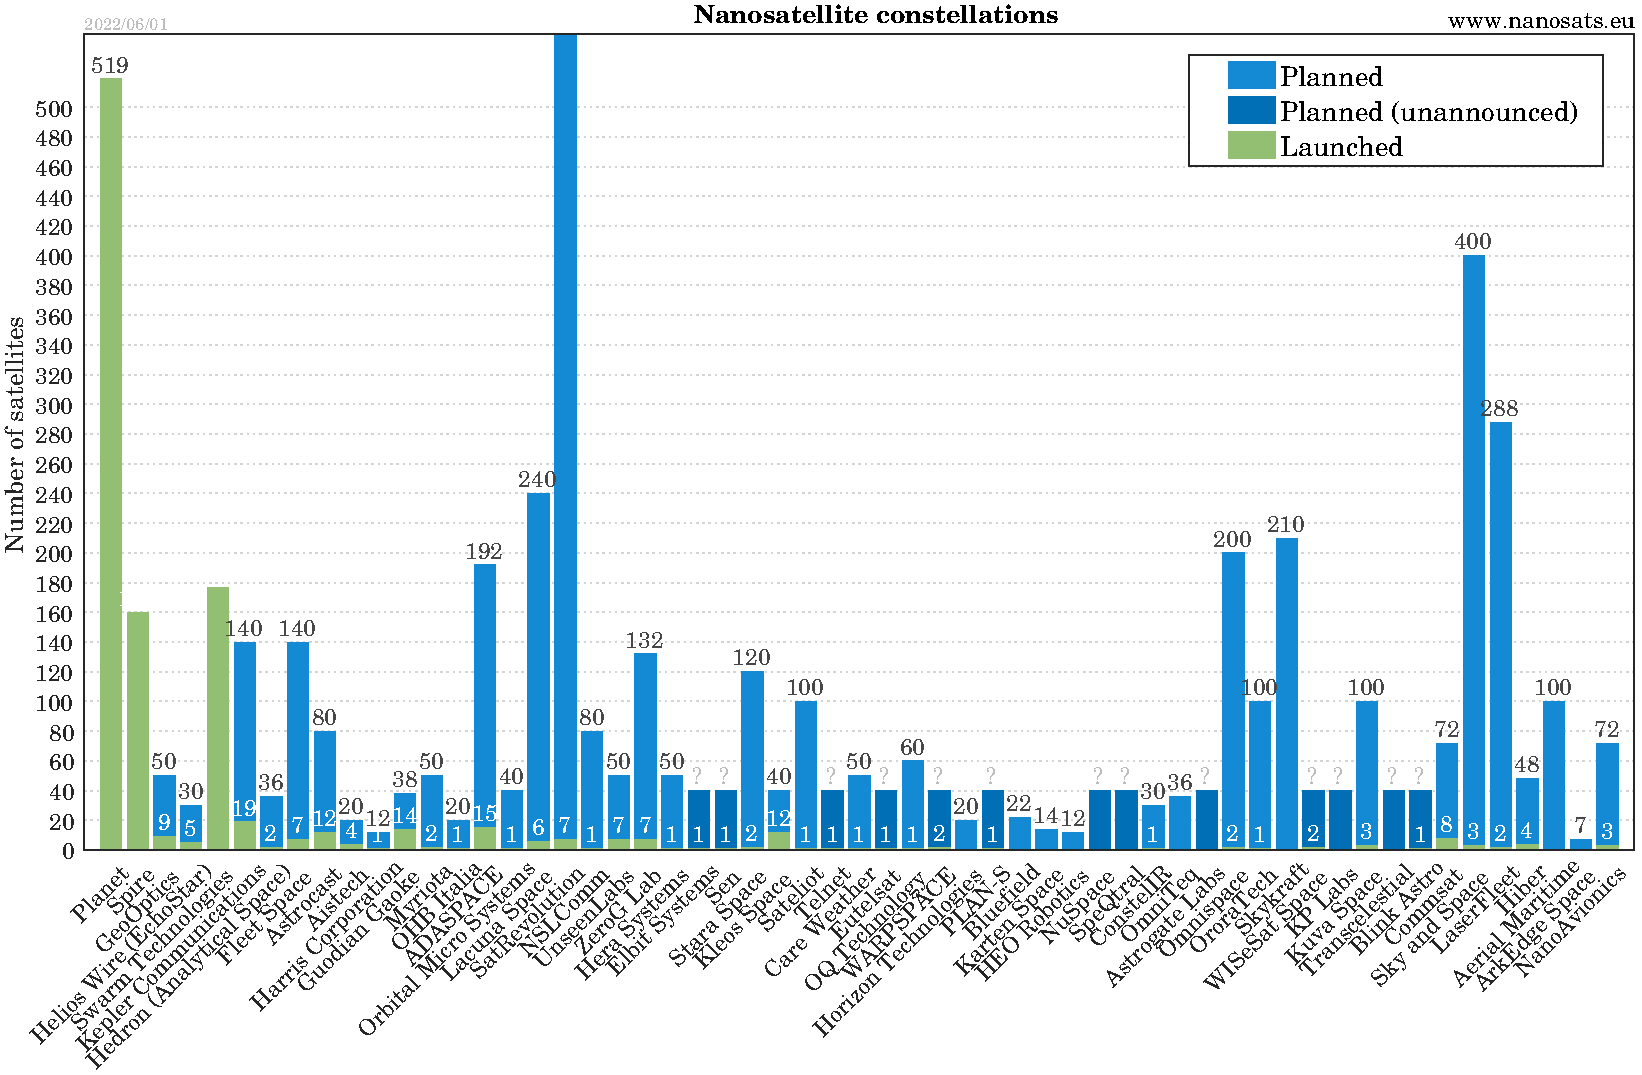
\includegraphics[width=\columnwidth]{figures/Nanosats_constellations_2022-06-01}
        \caption{Nanosatellite constellations (2022/06/01) \cite{nanosatseu}.}
        \label{fig:constellations}
    \end{center}
\end{figure}

\section{Motivation}

Considerando o contexto apresentado acima a respeito do crescimento atual da utilização de pequenos satélites e da implatação de constelações dos mesmos, e ainda o rápido crescimento de dispositivos com necessidade de conexão a internet, denominadados Internet das Coisas (ou \textit{Internet of Things}, IoT), e outras tipos de tecnologias em ascenção como veículos autônomos, uma possível utilização dos nanossatélites seria em sistemas de navegação e localização, seja de cobertura específica para uma área, ou com cobertura global (GNSS).

Atualmente, os sistemas de navegação por satélite são compostos por satélites de grande porte operando em altitudes elevadas, normalmente em órbitas médias (MEO) ou até em órbitas geoestacionárias. Como será apresentado neste trabalho, a utilização de satélites de pequeno porte neste tipo de aplicação pode trazer algumas vantagens como um menor custo de implantação e operação, uma maior cobertura territorial e maior precisão, e até mesmos a simplificação de receptores em terra.

\section{Organizaçao do trabalho}

O \autoref{ch:related-work} apresenta uma revisão do estado da arte, comentando sobre o funcionamento de cada uma das redes atuais de GNSS, e apresentando os principais trabalhos relacionados, tanto a respeito da utilização de pequenos satéltes para este tipo de aplicação, quanto a repeito de tecnologias específicas que poderiam ser utilizadas para uma rede deste tipo.

O \autoref{ch:problem-discussion} discure os principais problemas e questões a respeito da utilização de pequenos satélites e constelações dos mesmos para solucionar este tipo de problema. Neste capítulo apresenta-se possíveis tecnologias que poderiam ser utilizadas, questões de desempenho, entre outros.

Já o \autoref{ch:proposed-work}, apresenta de forma detalhada o trabalha proposto, discutindo-se as principais questões a serem levadas em consideração neste tipo de problema, possíveis soluções que podem ser exploradas e análises preliminares.
